% ============================================================
%   CHAPITRE : Calcul matriciel
%   Niveau   : Terminale S
%   Mazava Maths
% ============================================================
\chapter{Calcul matriciel}

\begin{objectifs}
	\begin{itemize}[label=\textbullet]
		\item Manipuler les matrices carrées : addition, produit par un scalaire, produit.
		\item Calculer déterminant, trace et puissance d'une matrice carrée.
		\item Déterminer si une matrice est inversible et calculer son inverse.
		\item Utiliser le calcul matriciel pour résoudre un système linéaire.
	\end{itemize}
\end{objectifs}


% ============================================================
\section{Définitions}
% ============================================================

\begin{definition}[Matrice carrée d'ordre $n$]
	Une \textbf{matrice carrée d'ordre $n$} est un tableau de $n^2$ nombres
	réels disposés en $n$ lignes et $n$ colonnes. On note :
	\[
	A = \bigl(a_{ij}\bigr)_{1\le i,j \le n}
	=
	\begin{pmatrix}
		a_{11} & a_{12} & \cdots & a_{1n} \\
		a_{21} & a_{22} & \cdots & a_{2n} \\
		\vdots & \vdots & \ddots & \vdots \\
		a_{n1} & a_{n2} & \cdots & a_{nn}
	\end{pmatrix}
	\]
	où $a_{ij}$ désigne l'élément situé à la \textbf{ligne $i$}, \textbf{colonne $j$}.
\end{definition}

\begin{center}
	\begin{tikzpicture}[>=stealth, font=\small]
		\matrix (M) [matrix of math nodes,
		left delimiter=(, right delimiter=),
		nodes={minimum width=1.6em, minimum height=1.6em, inner sep=4pt},
		row sep=2pt, column sep=2pt]
		{
			a_{11} & a_{12} & a_{13} \\
			a_{21} & a_{22} & a_{23} \\
			a_{31} & a_{32} & a_{33} \\
		};
		\draw[decorate, decoration={brace, amplitude=6pt, mirror}]
		(M-1-1.north west) -- (M-3-1.south west)
		node[midway, left=8pt] {lignes};
		\draw[decorate, decoration={brace, amplitude=6pt}]
		(M-1-1.north west) -- (M-1-3.north east)
		node[midway, above=8pt] {colonnes};
		\draw[->] (3,0.3) node[right] {$a_{ij}$ : ligne $i$, colonne $j$}
		-- (M-2-3.east);
	\end{tikzpicture}
\end{center}

\begin{definition}[Matrices particulières]
	On distingue en particulier :
	\begin{itemize}[label=\textbullet]
		\item \textbf{Matrice nulle} $O_n$ : tous les coefficients sont nuls.
		\item \textbf{Matrice identité} $I_n$ : $a_{ii}=1$ pour tout $i$,
		et $a_{ij}=0$ pour $i\neq j$ (matrice diagonale avec des $1$).
		\item \textbf{Matrice diagonale} : $a_{ij}=0$ pour tout $i\neq j$.
		\item \textbf{Matrice transposée} de $A$ : notée ${}^tA$, on échange
		lignes et colonnes — $({}^tA)_{ij} = a_{ji}$.
	\end{itemize}
\end{definition}

\begin{exemple}
	\[
	O_3 = \begin{pmatrix}0&0&0\\0&0&0\\0&0&0\end{pmatrix}, \quad
	I_3 = \begin{pmatrix}1&0&0\\0&1&0\\0&0&1\end{pmatrix}, \quad
	A   = \begin{pmatrix}2&-1&3\\0&4&1\\-2&0&5\end{pmatrix}, \quad
	{}^tA = \begin{pmatrix}2&0&-2\\-1&4&0\\3&1&5\end{pmatrix}.
	\]
\end{exemple}


% ============================================================
\section{Opérations sur les matrices carrées}
% ============================================================

\subsection{Addition et multiplication par un scalaire}

\begin{propriete}{Addition et scalaire}{}
	Soient $A=(a_{ij})$ et $B=(b_{ij})$ deux matrices d'ordre $n$,
	et $\lambda \in \R$.
	\begin{itemize}[label=\textbullet]
		\item \textbf{Somme :} $A+B = (a_{ij}+b_{ij})$ \quad
		(on additionne terme à terme).
		\item \textbf{Produit par un scalaire :} $\lambda A = (\lambda\,a_{ij})$.
		\item \textbf{Opposée :} $-A = (-a_{ij})$.
	\end{itemize}
	Ces opérations donnent encore une matrice d'ordre $n$.
\end{propriete}

\begin{exemple}
	\[
	A=\begin{pmatrix}1&2\\3&-1\end{pmatrix},\quad
	B=\begin{pmatrix}0&-2\\1&4\end{pmatrix}
	\implies
	A+B=\begin{pmatrix}1&0\\4&3\end{pmatrix},\quad
	2A=\begin{pmatrix}2&4\\6&-2\end{pmatrix}.
	\]
\end{exemple}

\subsection{Produit de deux matrices}

\begin{definition}[Produit matriciel]
	Soient $A=(a_{ij})$ et $B=(b_{ij})$ deux matrices d'ordre $n$.
	Le \textbf{produit} $C = AB$ est la matrice d'ordre $n$ définie par :
	\[
	c_{ij} = \sum_{k=1}^{n} a_{ik}\,b_{kj}
	= a_{i1}b_{1j} + a_{i2}b_{2j} + \cdots + a_{in}b_{nj}.
	\]
	L'élément $c_{ij}$ est le \textbf{produit scalaire} de la ligne $i$ de $A$
	par la colonne $j$ de $B$.
\end{definition}

\begin{center}
	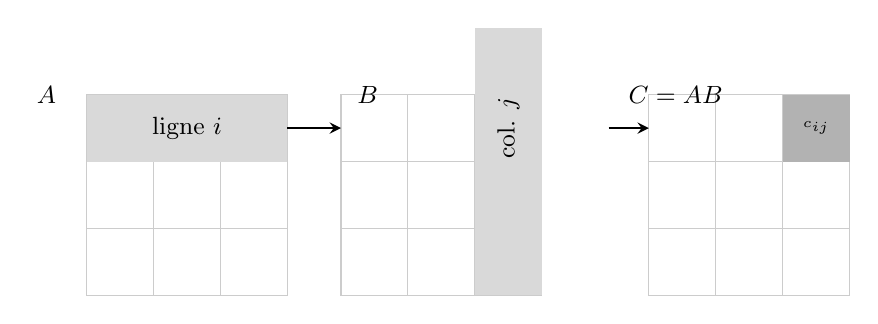
\begin{tikzpicture}[>=stealth, font=\small, scale=0.85]
		\foreach \i in {1,2,3}{
			\foreach \j in {1,2,3}{
				\draw[gray!40] (\j-1, -\i+0.5) rectangle (\j, -\i+1.5);
			}
		}
		\fill[black!15] (0,-0.5) rectangle (3,0.5);
		\node at (1.5, 0) {ligne $i$};
		\node at (-0.6, 0.5) {$A$};

		\foreach \i in {1,2,3}{
			\foreach \j in {1,2,3}{
				\draw[gray!40] (3.8+\j-1, -\i+0.5) rectangle (3.8+\j, -\i+1.5);
			}
		}
		\fill[black!15] (5.8,-2.5) rectangle (6.8,1.5);
		\node[rotate=90] at (6.3,0) {col. $j$};
		\node at (4.2, 0.5) {$B$};

		\foreach \i in {1,2,3}{
			\foreach \j in {1,2,3}{
				\draw[gray!40] (8.4+\j-1, -\i+0.5) rectangle (8.4+\j, -\i+1.5);
			}
		}
		\fill[black!30] (10.4,-0.5) rectangle (11.4,0.5);
		\node[font=\tiny] at (10.9, 0) {$c_{ij}$};
		\node at (8.8, 0.5) {$C=AB$};

		\draw[->, thick] (3,0) -- (3.8,0);
		\draw[->, thick] (7.8,0) -- (8.4,0);
	\end{tikzpicture}
\end{center}

\begin{attention}
	Le produit matriciel est \textbf{non commutatif} en général :
	$AB \neq BA$. Il faut toujours respecter l'ordre des facteurs.
\end{attention}

\begin{propriete}{Propriétés du produit}{}
	Pour toutes matrices carrées $A$, $B$, $C$ d'ordre $n$ et $\lambda\in\R$ :
	\begin{itemize}[label=\textbullet]
		\item \textbf{Associativité :} $(AB)C = A(BC)$.
		\item \textbf{Distributivité :} $A(B+C)=AB+AC$ et $(A+B)C=AC+BC$.
		\item \textbf{Élément neutre :} $AI_n = I_nA = A$.
		\item \textbf{Élément absorbant :} $AO_n = O_nA = O_n$.
		\item \textbf{Scalaire :} $(\lambda A)B = A(\lambda B) = \lambda(AB)$.
	\end{itemize}
\end{propriete}

\begin{exemple}
	\[
	A=\begin{pmatrix}1&2\\3&4\end{pmatrix},\quad
	B=\begin{pmatrix}0&1\\-1&2\end{pmatrix}.
	\]
	\[
	AB = \begin{pmatrix}1\cdot0+2\cdot(-1) & 1\cdot1+2\cdot2\\
		3\cdot0+4\cdot(-1) & 3\cdot1+4\cdot2\end{pmatrix}
	= \begin{pmatrix}-2&5\\-4&11\end{pmatrix}.
	\]
	\[
	BA = \begin{pmatrix}0\cdot1+1\cdot3 & 0\cdot2+1\cdot4\\
		-1\cdot1+2\cdot3 & -1\cdot2+2\cdot4\end{pmatrix}
	= \begin{pmatrix}3&4\\5&6\end{pmatrix}.
	\]
	Ainsi $AB \neq BA$ : le produit est bien non commutatif.
\end{exemple}

\begin{propriete}{Résumé : le produit matriciel}{}
	\begin{itemize}[label=\textbullet]
		\item \textbf{Condition :} pour des matrices carrées d'ordre $n$, le produit $AB$
		est toujours défini (plus généralement, pour des matrices rectangulaires,
		le nombre de colonnes de $A$ doit égaler le nombre de lignes de $B$).
		\item \textbf{Calcul :} $c_{ij}$ = ligne $i$ de $A$ « fois » colonne $j$ de $B$,
		soit $c_{ij} = \sum_{k=1}^n a_{ik}\,b_{kj}$.
		\item \textbf{Non commutatif :} en général $AB \neq BA$.
		\item \textbf{Associatif et distributif} par rapport à l'addition.
		\item \textbf{Élément neutre} $I_n$, \textbf{élément absorbant} $O_n$.
	\end{itemize}
\end{propriete}

\subsection{Puissance $n$-ième}

\begin{definition}[Puissance d'une matrice]
	Soit $A$ une matrice carrée d'ordre $n$ et $p\in\N^*$.
	\[
	A^p = \underbrace{A \times A \times \cdots \times A}_{p \text{ fois}}, \qquad
	A^0 = I_n.
	\]
\end{definition}

\begin{methode}
	\textbf{Calculer $A^n$ par récurrence :}
	\begin{enumerate}
		\item Calculer $A^2$, puis $A^3 = A^2 \cdot A$.
		\item Chercher une relation du type $A^2 = \alpha A + \beta I_n$.
		\item En déduire $A^n$ par récurrence ou substitution.
	\end{enumerate}
\end{methode}

\begin{astucebac}
	Si $A^2 = aA + bI_n$, alors $A^3 = A\cdot A^2 = a A^2 + bA
	= a(aA+bI_n)+bA = (a^2+b)A + abI_n$.
	On peut ainsi exprimer toute puissance de $A$ sous la forme $\alpha A + \beta I_n$.
\end{astucebac}

\subsection{Déterminant}

\begin{definition}[Déterminant d'ordre 2 et 3]
	\textbf{Ordre 2 :}
	\[
	\det\begin{pmatrix}a&b\\c&d\end{pmatrix} = ad - bc.
	\]
	\textbf{Ordre 3 (règle de Sarrus) :}
	\[
	\det\begin{pmatrix}a&b&c\\d&e&f\\g&h&i\end{pmatrix}
	= aei + bfg + cdh - ceg - bdi - afh.
	\]
\end{definition}

\begin{center}
	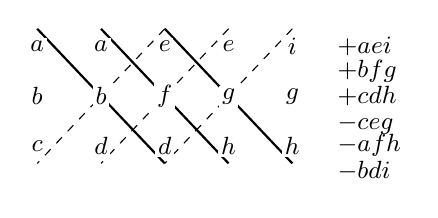
\begin{tikzpicture}[>=stealth, font=\small, scale=0.9]
		\def\el{{"a","b","c","a","b","d","e","f","d","e","g","h","i","g","h"}}
		\foreach \s in {0,1,2}{
			\draw[thick] (\s*0.9+0.0, 0.25) -- (\s*0.9+1.8, -1.65);
		}
		\foreach \s in {0,1,2}{
			\draw[dashed] (\s*0.9+1.8, 0.25) -- (\s*0.9+0.0, -1.65);
		}
		\foreach \j in {0,...,4}{
			\foreach \i in {0,1,2}{
				\pgfmathsetmacro\idx{int(\j*3+\i)}
				\pgfmathsetmacro\val{\el[\idx]}
				\node[fill=white, inner sep=1pt] at (\j*0.9, -\i*0.7) {$\val$};
			}
		}
		\node[right] at (4.1, 0)   {$+aei$};
		\node[right] at (4.1,-0.35){$+bfg$};
		\node[right] at (4.1,-0.7) {$+cdh$};
		\node[right] at (4.1,-1.1) {$-ceg$};
		\node[right] at (4.1,-1.4) {$-afh$};
		\node[right] at (4.1,-1.75){$-bdi$};
	\end{tikzpicture}
\end{center}

\begin{propriete}{Propriétés du déterminant}{}
	\begin{itemize}[label=\textbullet]
		\item $\det(AB) = \det(A)\cdot\det(B)$.
		\item $\det(A^n) = [\det(A)]^n$.
		\item $A$ est inversible $\iff \det(A) \neq 0$.
		\item $\det({}^tA) = \det(A)$.
	\end{itemize}
\end{propriete}

\subsection{Trace}

\begin{definition}[Trace]
	La \textbf{trace} de $A=(a_{ij})$ est la somme des termes diagonaux :
	\[
	\mathrm{tr}(A) = a_{11} + a_{22} + \cdots + a_{nn} = \sum_{i=1}^n a_{ii}.
	\]
\end{definition}

\begin{propriete}{Propriétés de la trace}{}
	\begin{itemize}[label=\textbullet]
		\item $\mathrm{tr}(A+B) = \mathrm{tr}(A)+\mathrm{tr}(B)$.
		\item $\mathrm{tr}(\lambda A) = \lambda\,\mathrm{tr}(A)$.
		\item $\mathrm{tr}(AB) = \mathrm{tr}(BA)$.
	\end{itemize}
\end{propriete}

\subsection{Matrice inverse}

\begin{definition}[Matrice inversible]
	Une matrice carrée $A$ d'ordre $n$ est dite \textbf{inversible} s'il existe
	une matrice $B$ telle que :
	\[
	AB = BA = I_n.
	\]
	On note alors $B = A^{-1}$. L'inverse est \textbf{unique}.
\end{definition}

\begin{theoreme}[Existence de l'inverse]
	$A$ est inversible $\iff \det(A) \neq 0$.
\end{theoreme}

\begin{methode}
	\textbf{Inverse d'une matrice $2\times 2$ :}
	Si $A=\begin{pmatrix}a&b\\c&d\end{pmatrix}$ avec $ad-bc\neq 0$, alors :
	\[
	A^{-1} = \frac{1}{ad-bc}\begin{pmatrix}d&-b\\-c&a\end{pmatrix}.
	\]
\end{methode}

\begin{methode}
	\textbf{Vérification de l'inverse (méthode BAC) :}
	Pour vérifier que $B=A^{-1}$ : calculer $AB$ et $BA$ et montrer
	que $AB = BA = I_n$.
\end{methode}

\begin{astucebac}
	Au BAC, l'inverse est souvent obtenu \textbf{par déduction} :
	si on montre que $\alpha A^2 + \beta A = \gamma I_n$,
	alors $A\bigl(\frac{\alpha}{\gamma}A + \frac{\beta}{\gamma}I_n\bigr) = I_n$,
	donc $A^{-1} = \frac{\alpha}{\gamma}A + \frac{\beta}{\gamma}I_n$.
\end{astucebac}

\begin{exemple}
	Soit $A = \begin{pmatrix}2&1\\5&3\end{pmatrix}$.
	$\det(A)=6-5=1\neq 0$ donc $A$ est inversible.
	\[
	A^{-1} = \frac{1}{1}\begin{pmatrix}3&-1\\-5&2\end{pmatrix}
	= \begin{pmatrix}3&-1\\-5&2\end{pmatrix}.
	\]
	\textbf{Vérification :}
	$AA^{-1}=\begin{pmatrix}2&1\\5&3\end{pmatrix}\begin{pmatrix}3&-1\\-5&2\end{pmatrix}
	=\begin{pmatrix}1&0\\0&1\end{pmatrix}=I_2.$
\end{exemple}


% ============================================================
\section{Application : résolution d'un système linéaire}
% ============================================================

\begin{methode}
	\textbf{Résolution matricielle d'un système :}
	Un système de $n$ équations à $n$ inconnues s'écrit sous forme matricielle :
	\[
	AX = B
	\]
	où $A$ est la matrice des coefficients, $X$ la matrice colonne des inconnues,
	$B$ la matrice colonne des seconds membres.

	Si $\det(A)\neq 0$, l'unique solution est :
	\[
	\boxed{X = A^{-1}B.}
	\]
\end{methode}

\begin{exemple}
	\[
	\begin{cases} 2x + y = 5 \\ 5x + 3y = 13 \end{cases}
	\implies
	\underbrace{\begin{pmatrix}2&1\\5&3\end{pmatrix}}_{A}
	\underbrace{\begin{pmatrix}x\\y\end{pmatrix}}_{X}
	=
	\underbrace{\begin{pmatrix}5\\13\end{pmatrix}}_{B}.
	\]
	Avec $A^{-1}=\begin{pmatrix}3&-1\\-5&2\end{pmatrix}$ (calculé ci-dessus) :
	\[
	X = A^{-1}B = \begin{pmatrix}3&-1\\-5&2\end{pmatrix}\begin{pmatrix}5\\13\end{pmatrix}
	= \begin{pmatrix}15-13\\-25+26\end{pmatrix}
	= \begin{pmatrix}2\\1\end{pmatrix}.
	\]
	Donc $x=2$ et $y=1$.
\end{exemple}


% ============================================================
\section{Exercices résolus}
% ============================================================

\exerciceresolu
\textbf{Utiliser une relation polynomiale pour inverser une matrice}

Soit $A = \begin{pmatrix}0&-1&-1\\-1&0&-1\\-1&-1&0\end{pmatrix}$.
\begin{enumerate}
	\item Calculer $A^2$ et $A^3$.
	\item Vérifier que $4A + A^2 - A^3 = 4I_3$.
	\item En déduire que $A$ est inversible et donner $A^{-1}$.
\end{enumerate}

\solution

\textbf{1. Calcul de $A^2$.}
\[
A^2 = A\cdot A =
\begin{pmatrix}0&-1&-1\\-1&0&-1\\-1&-1&0\end{pmatrix}
\begin{pmatrix}0&-1&-1\\-1&0&-1\\-1&-1&0\end{pmatrix}
= \begin{pmatrix}2&1&1\\1&2&1\\1&1&2\end{pmatrix}
\]
(en calculant chaque coefficient $c_{ij}=\sum_k a_{ik}a_{kj}$, et en utilisant la symétrie de $A$).

\textbf{Calcul de $A^3 = A^2 \cdot A$.}
\[
A^3 =
\begin{pmatrix}2&1&1\\1&2&1\\1&1&2\end{pmatrix}
\begin{pmatrix}0&-1&-1\\-1&0&-1\\-1&-1&0\end{pmatrix}
= \begin{pmatrix}-2&-3&-3\\-3&-2&-3\\-3&-3&-2\end{pmatrix}.
\]

\textbf{2. Vérification.}
\[
4A + A^2 - A^3
= \begin{pmatrix}0&-4&-4\\-4&0&-4\\-4&-4&0\end{pmatrix}
+ \begin{pmatrix}2&1&1\\1&2&1\\1&1&2\end{pmatrix}
- \begin{pmatrix}-2&-3&-3\\-3&-2&-3\\-3&-3&-2\end{pmatrix}
= \begin{pmatrix}4&0&0\\0&4&0\\0&0&4\end{pmatrix}
= 4I_3.
\]

\textbf{3. Déduction de $A^{-1}$.}

De $4A + A^2 - A^3 = 4I_3$, on factorise le membre gauche par $A$ :
\[
A\bigl(4I_3 + A - A^2\bigr) = 4I_3.
\]
On divise par $4$ :
\[
A \cdot \frac{1}{4}\bigl(4I_3 + A - A^2\bigr) = I_3.
\]
Donc $A$ est inversible et :
\[
A^{-1} = \frac{1}{4}(4I_3 + A - A^2)
= \frac{1}{4}\begin{pmatrix}2&-2&-2\\-2&2&-2\\-2&-2&2\end{pmatrix}.
\]
\[
\boxed{A^{-1} = \frac{1}{2}\begin{pmatrix}1&-1&-1\\-1&1&-1\\-1&-1&1\end{pmatrix}.}
\]

\exerciceresolu
\textbf{Vérifier un inverse et calculer une puissance par récurrence}

On considère les matrices :
\[
A = \begin{pmatrix}0&1&2\\1&3&0\\1&2&1\end{pmatrix}, \qquad
B = \frac{1}{3}\begin{pmatrix}-3&-3&6\\1&2&-2\\1&-1&1\end{pmatrix}, \qquad
C = \begin{pmatrix}2&2&0\\0&2&0\\0&0&2\end{pmatrix}.
\]
\begin{enumerate}
	\item Montrer que $B$ est l'inverse de $A$.
	\item Calculer $A+C$.
	\item Démontrer par récurrence que, pour tout $n\in\N^*\setminus\{1\}$ :
	\[
	C^n = \begin{pmatrix}2^n & n\cdot 2^n & 0\\0&2^n&0\\0&0&2^n\end{pmatrix}.
	\]
\end{enumerate}

\solution

\textbf{1. Vérification que $B = A^{-1}$.}

On calcule $AB$ :
\[
AB = \begin{pmatrix}0&1&2\\1&3&0\\1&2&1\end{pmatrix}
\cdot\frac{1}{3}\begin{pmatrix}-3&-3&6\\1&2&-2\\1&-1&1\end{pmatrix}
= \frac{1}{3}\begin{pmatrix}3&0&0\\0&3&0\\0&0&3\end{pmatrix} = I_3.
\]
De même $BA=I_3$. Ainsi $B = A^{-1}$.

\textbf{2. Calcul de $A+C$.}
\[
A+C = \begin{pmatrix}0+2&1+2&2+0\\1+0&3+2&0+0\\1+0&2+0&1+2\end{pmatrix}
= \begin{pmatrix}2&3&2\\1&5&0\\1&2&3\end{pmatrix}.
\]

\textbf{3. Récurrence sur $n$.}

\textit{Initialisation ($n=2$) :}
\[
C^2 = \begin{pmatrix}2&2&0\\0&2&0\\0&0&2\end{pmatrix}^2
= \begin{pmatrix}4&8&0\\0&4&0\\0&0&4\end{pmatrix}
= \begin{pmatrix}2^2&2\cdot2^2&0\\0&2^2&0\\0&0&2^2\end{pmatrix}.
\]

\textit{Hérédité :} Supposons que pour un certain $n\geq 2$ :
$C^n = \begin{pmatrix}2^n&n\cdot2^n&0\\0&2^n&0\\0&0&2^n\end{pmatrix}$.
Montrons la propriété au rang $n+1$ :
\[
C^{n+1} = C^n \cdot C
= \begin{pmatrix}2^n&n\cdot2^n&0\\0&2^n&0\\0&0&2^n\end{pmatrix}
\begin{pmatrix}2&2&0\\0&2&0\\0&0&2\end{pmatrix}
= \begin{pmatrix}2^{n+1}&(n+1)\cdot2^{n+1}&0\\0&2^{n+1}&0\\0&0&2^{n+1}\end{pmatrix}.
\]
La propriété est vraie au rang $n+1$. Par le principe de récurrence,
elle est vraie pour tout $n\in\N^*\setminus\{1\}$.

\exerciceresolu
\textbf{Résoudre un système linéaire à l'aide d'une matrice inverse donnée}

On considère le système $(S)$ :
\[
\begin{cases}
	3y + 2z = 7 \\
	x + y - z = 2 \\
	2x + y - 3z = 1
\end{cases}
\]
\begin{enumerate}
	\item Écrire $(S)$ sous forme matricielle $AX = B$.
	\item Soit $P = \begin{pmatrix}-2&11&-5\\1&-4&2\\-1&6&-3\end{pmatrix}$.
	Calculer $A\times P$ et $P\times A$. Conclure.
	\item En déduire la matrice $X$ (solution du système).
\end{enumerate}

\solution

\textbf{1. Forme matricielle.}
\[
A = \begin{pmatrix}0&3&2\\1&1&-1\\2&1&-3\end{pmatrix}, \quad
X = \begin{pmatrix}x\\y\\z\end{pmatrix}, \quad
B = \begin{pmatrix}7\\2\\1\end{pmatrix}, \quad
AX = B.
\]

\textbf{2. Calcul de $AP$.}
\[
AP =
\begin{pmatrix}0&3&2\\1&1&-1\\2&1&-3\end{pmatrix}
\begin{pmatrix}-2&11&-5\\1&-4&2\\-1&6&-3\end{pmatrix}
= \begin{pmatrix}1&0&0\\0&1&0\\0&0&1\end{pmatrix} = I_3.
\]
De même $PA = I_3$. Donc $P = A^{-1}$.

\textbf{3. Solution du système.}
\[
X = A^{-1}B = P\cdot B
= \begin{pmatrix}-2&11&-5\\1&-4&2\\-1&6&-3\end{pmatrix}
\begin{pmatrix}7\\2\\1\end{pmatrix}
= \begin{pmatrix}-14+22-5\\7-8+2\\-7+12-3\end{pmatrix}
= \begin{pmatrix}3\\1\\2\end{pmatrix}.
\]
\[
\boxed{x = 3, \quad y = 1, \quad z = 2.}
\]
